\section{Participatory Survey Results}
\label{sec:qual_results}

\subsection{User Experience about Data Deletion}

\begin{outlinenote}
talk about overall willingness of conducting data deletion, and impact of scenario sensitive on willingness of data deletion.  

talk about choices of data deletion methods, e.g., which one is most used, rarely used, and how scenario sensitivity will affect the choice.
\end{outlinenote}

In both scenarios, the majority of participants answered probably yes or definitely yes when asked whether they would delete the data (125 of 177 and 150 of 177), and they were more willing when the data were more sensitive. They also rated the method they chose as more protective in the more sensitive scenario, but not as more effortful or costly. So the more sensitive the data, the more users want to delete them, and the more protective they find their chosen method.

Participants relied on conversation-level deletion. Deleting a single conversation was both the most used method (136 of 177 participants) and the most chosen (46.6\% of 352 responses), and every method that acts on saved memories, an account, or a dashboard had been used by no more than a third of participants (Table~\ref{tab:method-use}). Filing a request was the least used (5 of 177). We found no change in which method participants chose between the scenarios. So sensitivity changes how much participants want to delete, not how they delete.

\begin{table*}[t]
\centering
\caption{Past use and choice of each data deletion method. Used is the number of the 177 participants who had used the method (select all that apply). Chosen is the number of responses naming the method, among the methods a participant had used, in each scenario and combined (352 responses from 176 participants; choices of Other are left out). Percentages are of 177 for Used and of 352 for Chosen.}
\label{tab:method-use}
\small
\begin{tabular}{@{}lrrrr@{}}
\toprule
Method & Used & Less & More & Chosen \\
\midrule
Sending a deletion-request prompt & 55 (31.1\%) & 25 & 14 & 39 (11.1\%) \\
Deleting a single conversation & 136 (76.8\%) & 84 & 80 & 164 (46.6\%) \\
Clearing all conversation history & 94 (53.1\%) & 33 & 40 & 73 (20.7\%) \\
Deleting a specific saved memory & 57 (32.2\%) & 19 & 22 & 41 (11.6\%) \\
Clearing all saved memories & 45 (25.4\%) & 7 & 8 & 15 (4.3\%) \\
Using a privacy dashboard & 17 (9.6\%) & 6 & 9 & 15 (4.3\%) \\
Deleting the account & 18 (10.2\%) & 2 & 3 & 5 (1.4\%) \\
Filing a request & 5 (2.8\%) & 0 & 0 & 0 (0.0\%) \\
\bottomrule
\end{tabular}
\end{table*}

\subsection{User Expectation about Data Deletion}

\para{Data deletion methods differ in efforts, but not protection, and benefit loss.}

Participants rated the four most chosen methods differently on effort, but not on protection or benefit loss (Figure~\ref{fig:scales}). Deleting a specific saved memory took the most effort and deleting a single conversation the least (mean ratings 2.49 and 1.64 on the five-point scale), while we found no difference between the methods in protection or benefit loss. So participants who reach into saved memories pay for it in effort, and we found no protection to show for it.

\begin{figure*}[t]
    \centering
    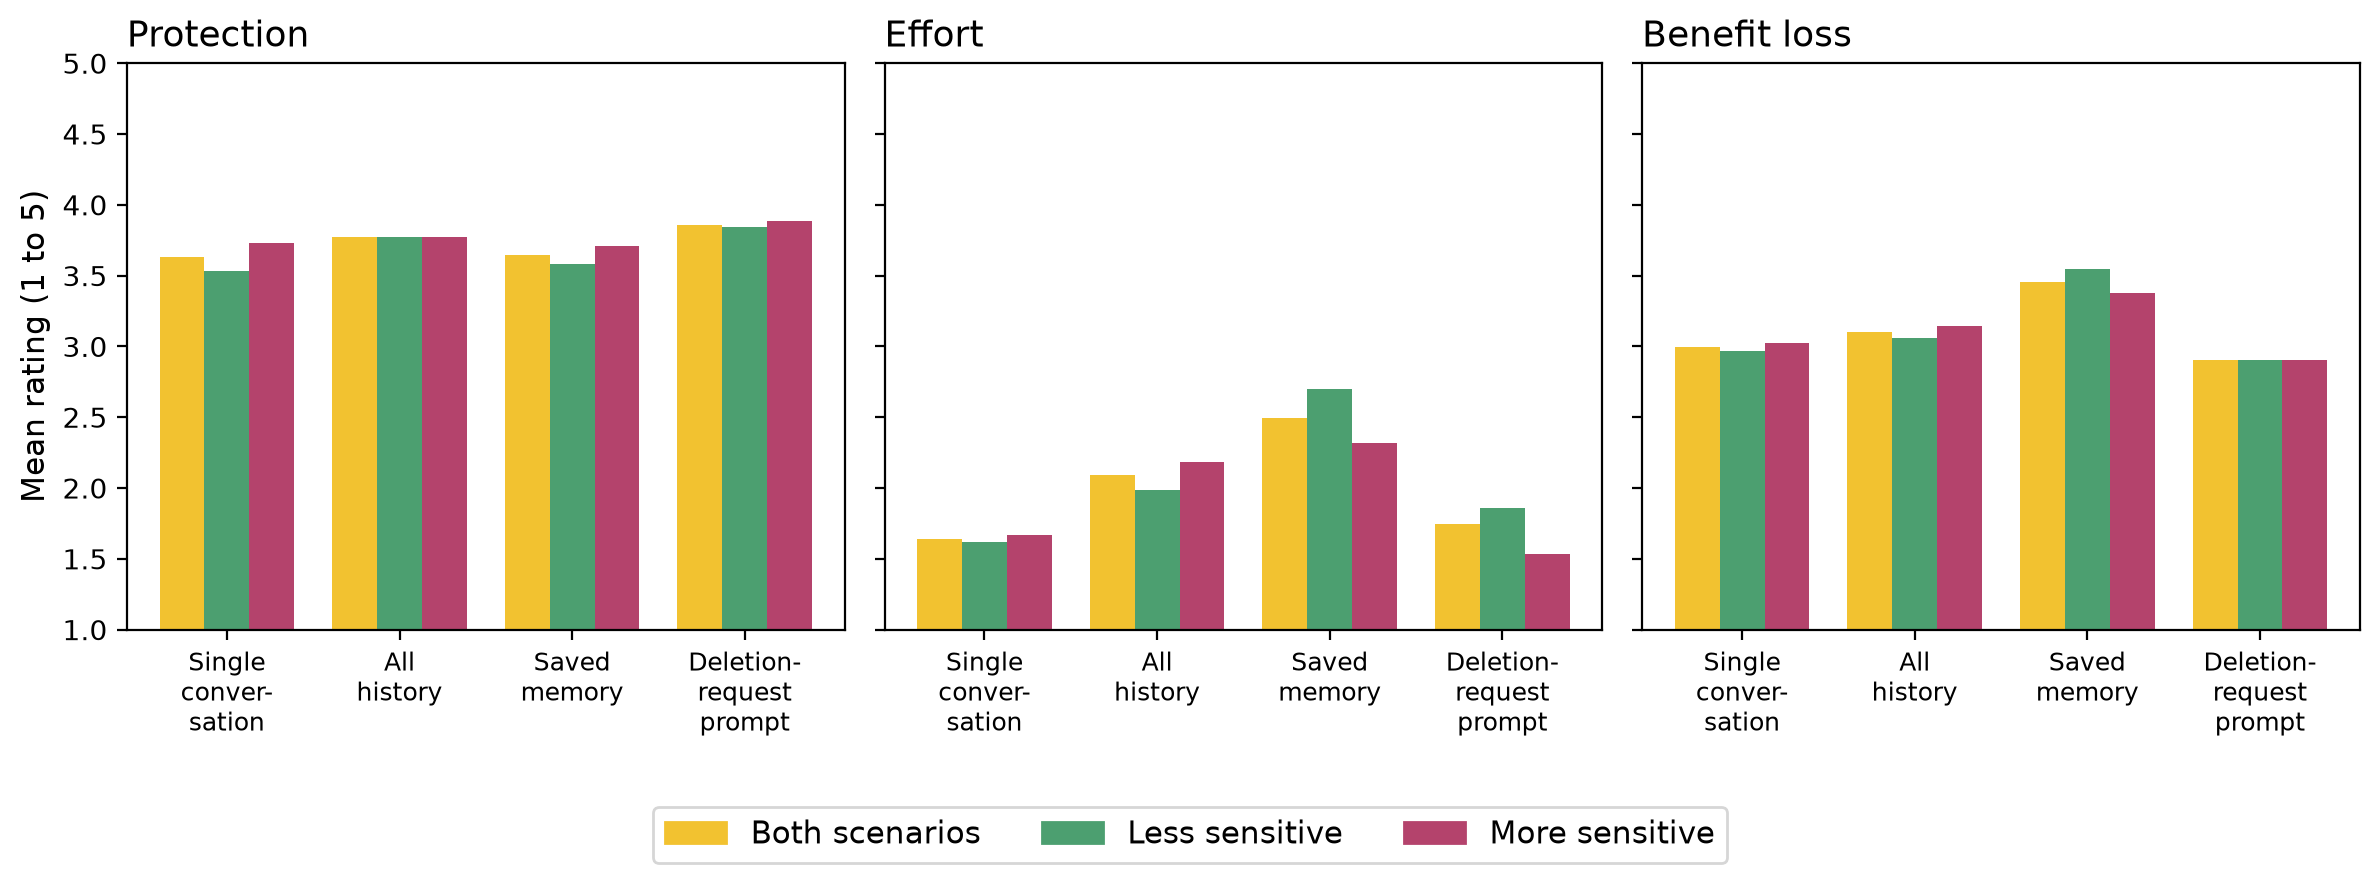
\includegraphics[width=0.9\textwidth]{figures/fig_scales.png}
    \caption{Mean ratings of protection, effort, and benefit loss for the four most chosen methods, for both scenarios combined and for each scenario (317 responses from 105, 50, 30, and 29 participants). Ratings use five-point agreement scales.}
    \label{fig:scales}
\end{figure*}


\para{Participants expect permanent deletion but can not check it.}

Most participants expected deletion to be permanent, but many could not check that it was (Figure~\ref{fig:expectation}). Across both scenarios, 59.0\% of responses expected permanent deletion from the database and backups, while 44.6\% said the participant did not know how to check. Asking the agent in the same conversation was the usual check for participants who deleted by sending a deletion-request prompt (53.8\% of those responses), and an unusual one for participants who deleted a single conversation (12.8\%). So users expect deletion to be final and have few ways to confirm it, and those who delete by asking the agent confirm it by asking the agent again.

\begin{figure}[t]
    \centering
    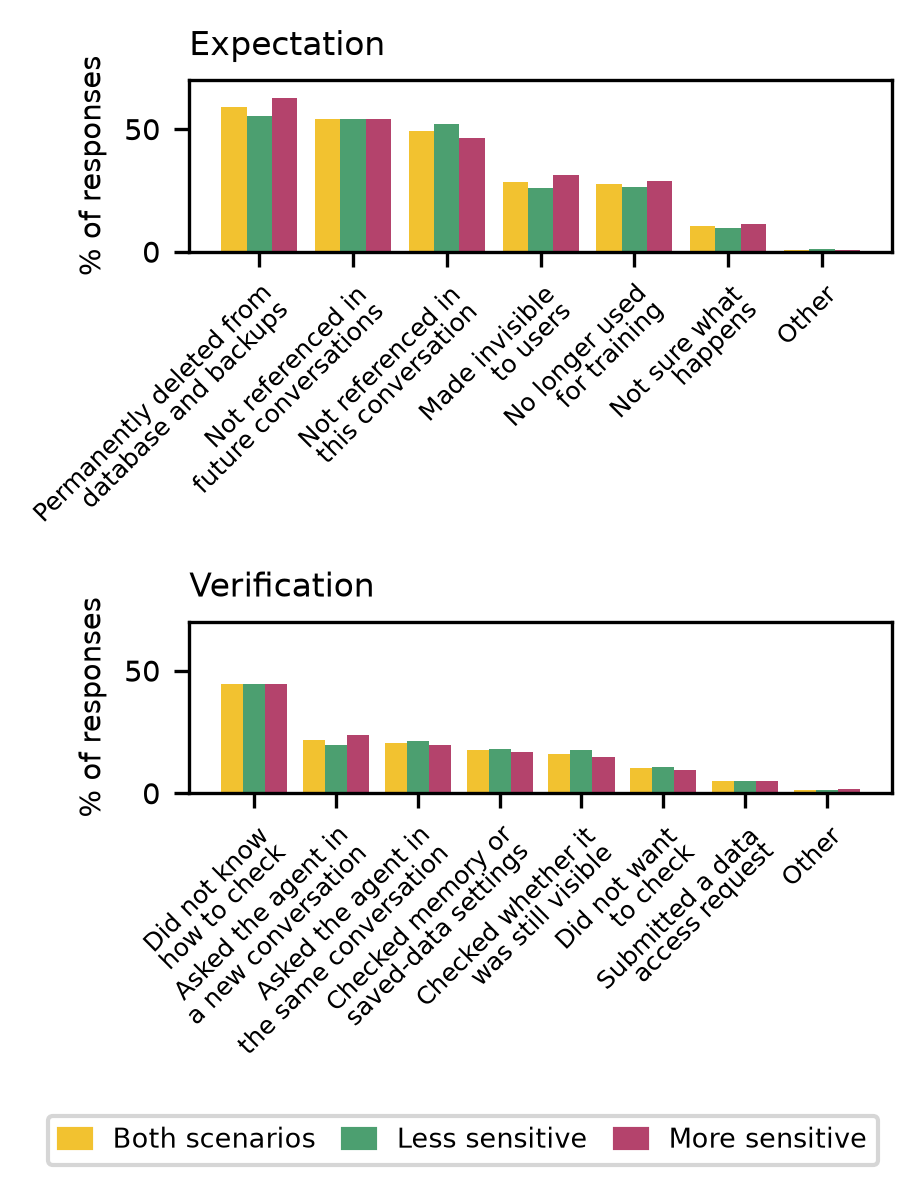
\includegraphics[width=\columnwidth,height=0.42\textheight,keepaspectratio]{figures/fig_expectation.png}
    \caption{Expectations of what deletion does, and how participants checked that it worked, in both scenarios combined and in each scenario (354 responses from 177 participants; participants could select several options). Percentages are of the 354 responses for both scenarios combined and of 177 for each scenario.}
    \label{fig:expectation}
\end{figure}

